\section{Auto-correlation and Peak Detection}

This section explains the crucial steps of auto-correlation and peak detection, which are essential in determining the BPM from the preprocessed audio signal.

\subsection{Auto-correlation to Identify Periodicity}

Auto-correlation is used to identify the periodicity within the smoothed energy signal, which is a crucial step for rhythm detection. It measures the similarity of the signal with itself at different time lags, highlighting the regular pattern of beats. Utilizing the \texttt{xcorr} function, the project computes the auto-correlation sequence, efficiently revealing the temporal intervals with high similarity — indicative of the periodic nature of beats.

\subsection{Overview of the \texttt{xcorr} Function Algorithm}

The \texttt{xcorr} function is pivotal in signal processing, providing a means to compute the cross-correlation of two signals, or the autocorrelation of a single signal. This function can handle both real and complex data, in vector or matrix form, making it versatile for a range of applications.

\subsubsection{Functionality}

\texttt{xcorr} estimates the similarity between two signals (\(X\) and \(Y\)) over a range of time lags. For a single input vector (\(X\)), it calculates the signal's autocorrelation. When \(X\) is a matrix, it performs cross-correlation across columns, treating each as an individual signal.

\subsubsection{Core Algorithm}

The cross-correlation between \(X\) and \(Y\) for a lag \(k\) is defined as:

\[
R_{xy}(k) = \sum_{i=1}^{N} x_{i+k} \cdot \text{conj}(y_i)
\]

where \(N\) is the signal length, and \(\text{conj}(y_i)\) denotes the complex conjugate of \(y_i\). The function fills missing data (e.g., \(x(-1)\), \(y(N+1)\)) with zeros. 

\subsubsection{Parameters}

\begin{itemize}
    \item \textbf{X, Y}: Input data vectors or matrices. If \(X\) is a matrix, \(Y\) must be omitted.
    \item \textbf{maxlag}: An integer specifying the maximum lag at which to calculate the correlation. If omitted, it defaults to \(N-1\).
    \item \textbf{scale}: A string indicating the scaling of the correlation output, with options including 'none', 'biased', 'unbiased', and 'coeff'.
\end{itemize}

\subsubsection{Computational Approach}

\texttt{xcorr} employs a spectral method for efficiency, utilizing the Fast Fourier Transform (FFT) to calculate correlations across the specified range of lags. This method is particularly effective for large datasets, as the computational effort is independent of the number of lags.

\subsubsection{Output}

The function returns \(R\), an array of correlation estimates across the specified lags, and \(lags\), a vector indicating the corresponding lag values.

\subsection{Peak Detection}

After determining the periodicity, the project proceeds to identify the major peaks in the auto-correlation function, which directly correspond to the timing of the beats. The \texttt{findpeaks} function is invoked to discern the prominent peaks from the auto-correlation sequence, with parameters fine-tuned to discern genuine beat-related peaks from noise.

\subsection{Overview of the \texttt{findpeaks} Function}

The \texttt{findpeaks} function is designed to identify local maxima in a given set of data, a common requirement in signal processing and time series analysis. It operates on continuous-valued data arrays, optionally filtered by a specified threshold, to pinpoint peak locations.

\subsubsection{Function Syntax}

\texttt{findpeaks} is invoked with the syntax:

\begin{verbatim}
    xmax = findpeaks(data, threshold)
\end{verbatim}

where \texttt{data} represents the input signal, and \texttt{threshold} is an optional parameter that specifies a minimum value peaks must exceed to be considered.

\subsubsection{Parameters}

\begin{itemize}
    \item \textbf{data}: A vector or matrix containing the signal data. If \texttt{data} is a matrix, it is treated as time x channels/trials, allowing for simultaneous peak detection across multiple channels or trials.
    \item \textbf{threshold} (optional): A scalar specifying the minimum value that data points must exceed to be identified as peaks. If omitted, all local maxima are returned.
\end{itemize}

\subsubsection{Algorithmic Approach}

The function identifies peaks by comparing each data point to its neighbors:
\begin{itemize}
    \item For a point to be considered a peak, it must be greater than its immediate neighbors. This is determined by subtracting the values of preceding (\texttt{pp1}) and following (\texttt{pp2}) points from the current point and checking if the result is positive.
    \item If a \texttt{threshold} is specified, a data point must also exceed this value to be labeled as a peak.
\end{itemize}

\subsubsection{Outputs}

\texttt{findpeaks} returns \texttt{xmax}, a structure array with fields corresponding to each channel/trial in the input \texttt{data}. Each field contains the locations (indices) of the local maxima detected.

\subsubsection{Usage Considerations}

\begin{itemize}
    \item The function is versatile, applicable to single vectors or multi-channel/time-series data, making it suitable for a wide range of applications in signal and data analysis.
    \item Specifying a \texttt{threshold} can help in filtering out noise and focusing on significant peaks.
\end{itemize}

\subsection{Graphical Analysis}

The graph below visually represents the process of auto-correlation and subsequent peak detection. It plots the normalized auto-correlation function (ACF) against time lag in seconds. The ACF is depicted in blue, showing how the signal's similarity with itself varies over different lags. Detected peaks are marked in red, indicating significant rhythmic patterns identified by the peak detection algorithm. The green line represents the dynamic threshold, which is a linear function used to determine the minimum threshold for beat detection. This threshold is crucial for distinguishing genuine rhythmic peaks from noise, ensuring that only significant peaks are considered in the estimation of BPM.

\begin{figure}[H]
    \centering
    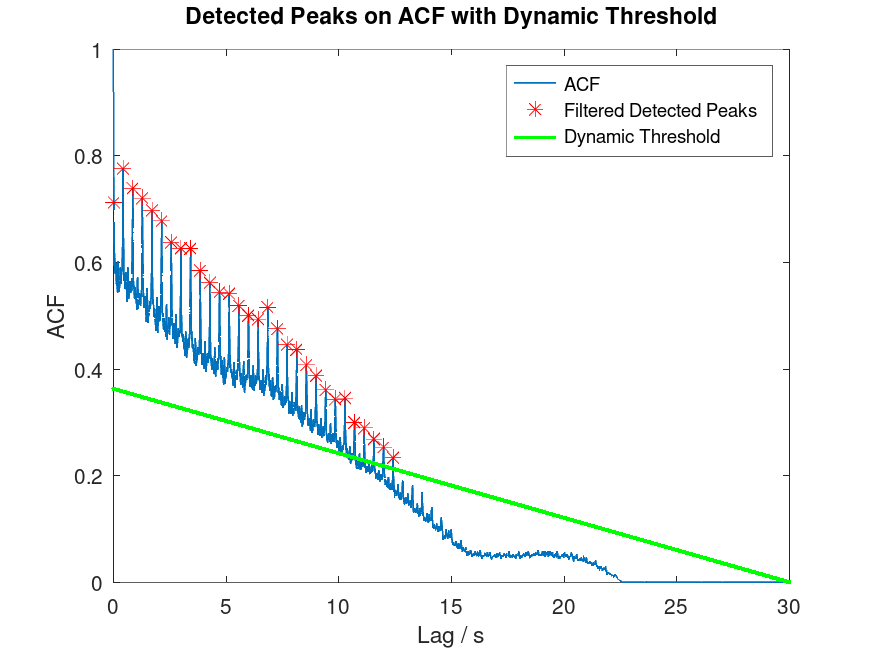
\includegraphics[width=0.8\textwidth]{peaks.png}
    \caption{Normalized Auto-correlation Function (ACF) with detected peaks and dynamic threshold.}
\end{figure}

\subsubsection{Decline of the ACF with Increasing Lag}

The ACF usually decreases as the lag increases, as shown in the graph. This decrease is due to the decreasing similarity between the signal and its shifted versions as the lag increases. At short lags, there is a higher likelihood of significant overlap between portions of the signal, resulting in higher correlation values. As the lag increases, the overlap decreases, leading to a decrease in correlation. The ACF's characteristic behavior is useful for identifying periodic beats in audio signals, as true rhythmic patterns tend to produce prominent peaks in the ACF at consistent intervals.

The relationship between auto-correlation and peak detection is fundamental to the process of estimating BPM. Auto-correlation reveals the inherent periodicity of the signal, which forms the basis for accurately identifying beats through peak detection. The dynamic threshold is crucial in this process, as it ensures that only peaks representing genuine rhythmic content are used in the final BPM calculation. This study's methodological rigor enhances the accuracy of BPM estimation, affirming the project's adaptability to various musical genres and demonstrating a robust approach to beat detection.

\subsection{Discussion}

The synergy between auto-correlation and peak detection is fundamental to BPM estimation. Auto-correlation reveals the signal's inherent periodicity, which enables the precise identification of beats through peak detection. The use of \texttt{xcorr} and \texttt{findpeaks}, with their FFT and gradient-based algorithms respectively, highlights the methodological rigor in capturing the essence of rhythm. This approach enhances accuracy and affirms the project's adaptability to the multifaceted nature of audio signals, ensuring reliable BPM estimation across diverse musical genres.
